\subsection{その他}
\subsubsection{ゆうきELディスプレイ}\label{oled}
\begin{table}[H]
	\begin{tabular}{|p{\colF}|p{\colG}|}	\hline
	名称 & 有機ELディスプレイ(ゆうきいーえるでぃすぷれい)\\ \hline
	接続箇所 & I2C (4pin)\\ \hline
	機能概要 & 文字の表示\\ \hline
  \end{tabular}
\end{table}

\begin{table}[H]
	\begin{tabular}{|p{\colF}|p{\colG}|}	\hline
	サンプルコードの場所 & 05/oled.hsp\\ \hline
	raspiへの入力 & なし\\ \hline
	raspiへの入力方法 & なし\\ \hline
	raspiからの出力 & プログラムで決めた文字や記号を表示する\\ \hline
	raspiからの出力方法 & oled “表示させたい文字”\\ \hline
  \end{tabular}
\end{table}

\begin{table}[H]
	\begin{tabular}{|p{\colF}|p{\colG}|} \hline
	使い道 & テレビ\\ \hline
	注意事項 & 日本語表示させることはできないので注意\\ \hline
	補足 & なし\\ \hline
  \end{tabular}
\end{table}

\begin{figure}[H]
	\begin{tabular}{|p{\colH}|p{\colI}|p{\colH}|p{\colI}|} \hline
	外観 & 
	\begin{minipage}[t]{\linewidth}
    \smallskip
      \centering
      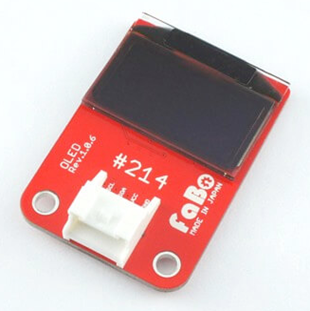
\includegraphics[width=\linewidth]{images/chap05/text05-img032.png}
      \caption{ゆうきELディスプレイ}
      \smallskip
    \end{minipage} &
    回路記号 & なし\\ \hline
  \end{tabular}
\end{figure}
